% Figure: a local multi-fragment XMI development setting next to a decentralized
% one. Panel (a) ties the fragments to one location, which can be a local disk,
% a shared network drive or an HTTP service. Panel (b) places the fragments in
% the cloud of the IPFS network, where no single location holds the content.
% Standalone TikZ source. The colors match the other figures: grey for mutable
% files, blue for immutable blocks and orange for a mutable name.
\documentclass[tikz,border=2pt]{standalone}
\usetikzlibrary{arrows.meta,calc,shapes.geometric,shapes.symbols}

\definecolor{ink}{HTML}{0B0B0B}
\definecolor{inksoft}{HTML}{52514E}
\definecolor{muted}{HTML}{898781}
\definecolor{mutablefill}{HTML}{F0EFEC}
\definecolor{immutablefill}{HTML}{CDE2FB}
\definecolor{immutableborder}{HTML}{1C5CAB}
\definecolor{pointerfill}{HTML}{FBE1D6}
\definecolor{pointerborder}{HTML}{B8501F}
\definecolor{cloudfill}{HTML}{F3F7FC}

\begin{document}
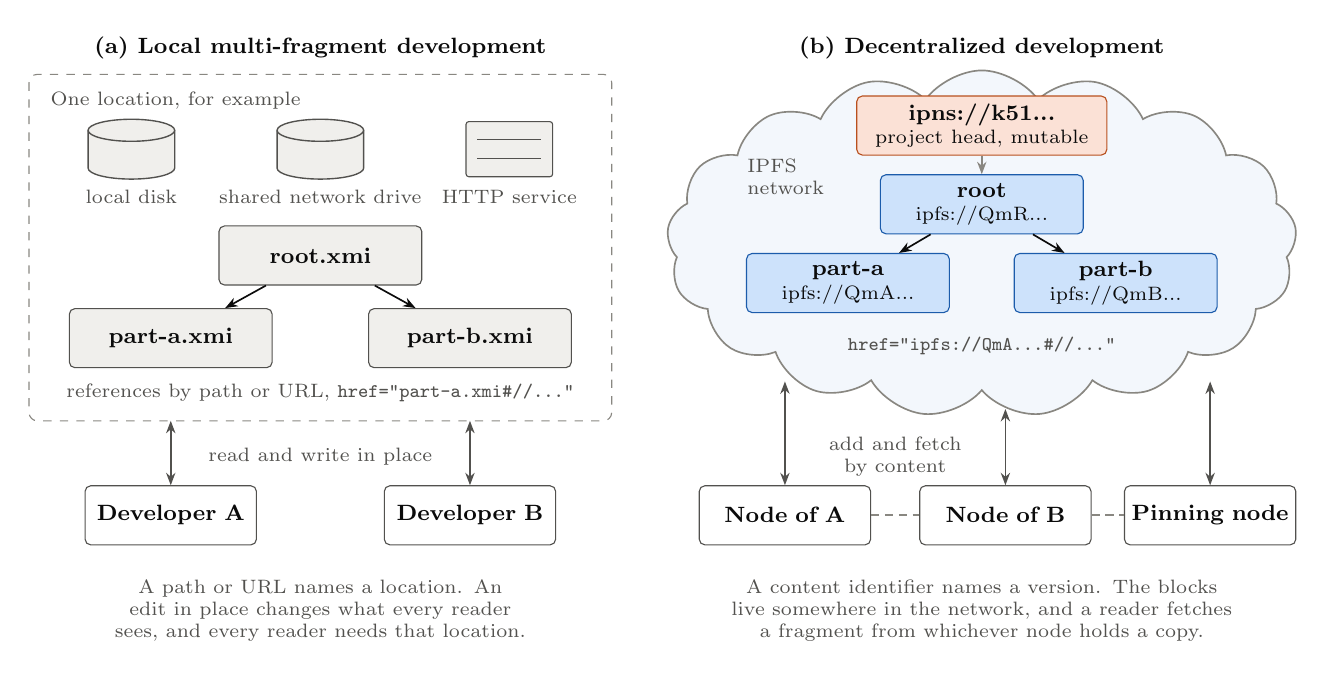
\begin{tikzpicture}[
  font={\footnotesize\hyphenpenalty=10000},
  >={Stealth[length=4.5pt]},
  box/.style={rounded corners=2pt, text=ink, align=center, inner sep=2.5pt,
    minimum height=7.5mm, text width=24mm},
  file/.style={box, draw=inksoft, fill=mutablefill},
  block/.style={box, draw=immutableborder, fill=immutablefill},
  pointer/.style={box, draw=pointerborder, fill=pointerfill, text width=30mm},
  actor/.style={box, draw=inksoft, fill=white, text width=20mm},
  diskicon/.pic={
    \draw[draw=inksoft, fill=mutablefill, line width=0.5pt]
      (-5.5mm,2.4mm) -- (-5.5mm,-2.4mm)
      arc[start angle=180, end angle=360, x radius=5.5mm, y radius=1.4mm] -- (5.5mm,2.4mm);
    \draw[draw=inksoft, fill=mutablefill, line width=0.5pt] (0,2.4mm) ellipse (5.5mm and 1.4mm);
  },
  server/.style={draw=inksoft, fill=mutablefill, rounded corners=1pt,
    minimum width=11mm, minimum height=7mm, inner sep=0pt},
  container/.style={draw=muted, dashed, rounded corners=3pt},
  ref/.style={->, draw=ink, line width=0.6pt},
  access/.style={<->, draw=inksoft, line width=0.6pt},
  soft/.style={->, draw=muted, line width=0.6pt},
  peer/.style={draw=muted, line width=0.6pt, densely dashed},
  paneltitle/.style={font=\footnotesize\bfseries, text=ink, anchor=north},
  small/.style={font={\scriptsize\hyphenpenalty=10000}, text=inksoft, align=center},
  note/.style={font={\scriptsize\hyphenpenalty=10000\exhyphenpenalty=10000}, text=inksoft,
    align=center, text width=72mm, anchor=north}
]

% ---------------------------------------------------------------------------
% (a) Local multi-fragment development: the fragments sit at one location
% ---------------------------------------------------------------------------
\node[paneltitle] at (37mm,0) {(a) Local multi-fragment development};

\draw[container] (0,-6mm) rectangle (74mm,-50mm);
\node[small, anchor=north west] at (1.5mm,-7mm) {One location, for example};

\pic at (13mm,-15.5mm) {diskicon};
\node[small] at (13mm,-21.5mm) {local disk};
\pic at (37mm,-15.5mm) {diskicon};
\node[small] at (37mm,-21.5mm) {shared network drive};
\node[server] (http) at (61mm,-15.5mm) {};
\draw[draw=inksoft, line width=0.4pt] ($(http.west)+(1.5mm,1.2mm)$) -- ($(http.east)+(-1.5mm,1.2mm)$);
\draw[draw=inksoft, line width=0.4pt] ($(http.west)+(1.5mm,-1.2mm)$) -- ($(http.east)+(-1.5mm,-1.2mm)$);
\node[small] at (61mm,-21.5mm) {HTTP service};

\node[file] (root) at (37mm,-29mm) {\textbf{root.xmi}};
\node[file] (pa) at (18mm,-39.5mm) {\textbf{part-a.xmi}};
\node[file] (pb) at (56mm,-39.5mm) {\textbf{part-b.xmi}};
\draw[ref] (root) -- (pa);
\draw[ref] (root) -- (pb);
\node[small] at (37mm,-46.5mm) {references by path or URL, \texttt{href="part-a.xmi\#//..."}};

\node[actor] (devA) at (18mm,-62mm) {\textbf{Developer A}};
\node[actor] (devB) at (56mm,-62mm) {\textbf{Developer B}};
\draw[access] (devA.north) -- (devA.north|-0,-50mm);
\draw[access] (devB.north) -- (devB.north|-0,-50mm);
\node[small] at (37mm,-54.5mm) {read and write in place};

\node[note] at (37mm,-69mm) {A path or URL names a location. An edit in place changes what every reader sees, and every reader needs that location.};

% ---------------------------------------------------------------------------
% (b) Decentralized development: the fragments sit in the IPFS network
% ---------------------------------------------------------------------------
\begin{scope}[xshift=84mm]
\node[paneltitle] at (37mm,0) {(b) Decentralized development};

\node[cloud, cloud puffs=17, cloud puff arc=110, aspect=1.75, draw=muted, fill=cloudfill,
  line width=0.6pt, minimum width=80mm, minimum height=44mm] (net) at (37mm,-27.5mm) {};
\node[small, anchor=west, align=left] at (6mm,-19mm) {IPFS\\network};

\node[pointer] (head) at (37mm,-12.5mm) {\textbf{ipns://k51...}\\[-1pt]\scriptsize project head, mutable};
\node[block] (croot) at (37mm,-22.5mm) {\textbf{root}\\[-1pt]\scriptsize ipfs://QmR...};
\node[block] (cpa) at (20mm,-32.5mm) {\textbf{part-a}\\[-1pt]\scriptsize ipfs://QmA...};
\node[block] (cpb) at (54mm,-32.5mm) {\textbf{part-b}\\[-1pt]\scriptsize ipfs://QmB...};
\draw[soft] (head) -- (croot);
\draw[ref] (croot) -- (cpa);
\draw[ref] (croot) -- (cpb);
\node[small] at (37mm,-40.5mm) {\texttt{href="ipfs://QmA...\#//..."}};

\node[actor] (nA) at (12mm,-62mm) {\textbf{Node of A}};
\node[actor] (nB) at (40mm,-62mm) {\textbf{Node of B}};
\node[actor] (nP) at (66mm,-62mm) {\textbf{Pinning node}};
\draw[access] (nA.north) -- (nA.north|-0,-45mm);
\draw[access] (nB.north) -- (nB.north|-0,-48.5mm);
\draw[access] (nP.north) -- (nP.north|-0,-45mm);
\draw[peer] (nA) -- (nB);
\draw[peer] (nB) -- (nP);
\node[small] at (26mm,-54.5mm) {add and fetch\\by content};

\node[note] at (37mm,-69mm) {A content identifier names a version. The blocks live somewhere in the network, and a reader fetches a fragment from whichever node holds a copy.};
\end{scope}

\end{tikzpicture}
\end{document}
